% !TEX program = xelatex

% Základní balíčky
\documentclass[10pt,a4paper]{article}
\usepackage[utf8]{inputenc}
\usepackage[T1]{fontenc}
\usepackage{graphicx}
\usepackage{wrapfig}
\usepackage{nonfloat}
\usepackage{amsmath}
\usepackage{hyperref}
\usepackage{gensymb}
\usepackage[top = 1cm, bottom = 1cm, left = 1cm, right = 1cm]{geometry}

% Language-related
\usepackage[czech]{babel}
\usepackage{csquotes}
\usepackage{polyglossia}
\setmainlanguage{czech}
\setotherlanguage{greek}

% Bibtex je oficiálně mrtka
% \usepackage[backend=bibtex,style=verbose-trad2]{biblatex}
% \usepackage{etoolbox}
% \patchcmd{\thebibliography}{\section*{\refname}}{}{}{}
% \bibliography{protokol}

% Pro titulní stránku
\usepackage{titlesec}
\usepackage{setspace}
\usepackage{framed}
\usepackage{array}

% Vlastní balíčky
\usepackage{gnuplottex}
\usepackage{epstopdf}
\usepackage{csvsimple}
\usepackage{units}
\usepackage{subfig}
\usepackage{pdfpages}

\usepackage{soul}

\usepackage{calc}
\newcommand*{\mask}[2]{\mathord{\makebox[\widthof{\(#1\)}]{\(#2\)}}}




\renewcommand{\U}[1]{\ensuremath{\,\mathrm{#1}}}
\newcommand{\°}{\degree}

\newcommand{\titjmeno}{Michal Grňo}
\newcommand{\titobor}{FOF}


\newcommand{\titcislo}{A1}
\newcommand{\titnazev}{Objevování částic v detektoru ATLAS v CERN}
\newcommand{\titmereni}{18. 11. 2020}
\newcommand{\titodevzdani}{2. 12. 2020}


\renewcommand{\t}[1]{\mathrm{#1}}


\newcommand{\Jpsi}{\ensuremath{J \hspace{-2pt} / \hspace{-1pt} \psi}}

\begin{document}


\thispagestyle{empty}
\newgeometry{top = 2.5cm, bottom = 0cm, left = 2.5cm, right = 3cm}

{%T tomto je uzavřena celá titulka
%Tloušťka rámečku
\setlength{\fboxrule}{1.5pt}

\noindent
\framebox{
\begin{minipage}{\textwidth}
\setlength{\parindent}{17.62482 pt}
\phantom{d}

\begin{minipage}{0.6\textwidth}
{
\Large Kabinet výuky obecné fyziky, UK MFF\\
}
\vspace*{0.2cm}

{
\bfseries
\huge Fyzikální praktikum %ČÍSLO
}
\end{minipage}
\begin{minipage}{0.4\textwidth}
\begin{center}
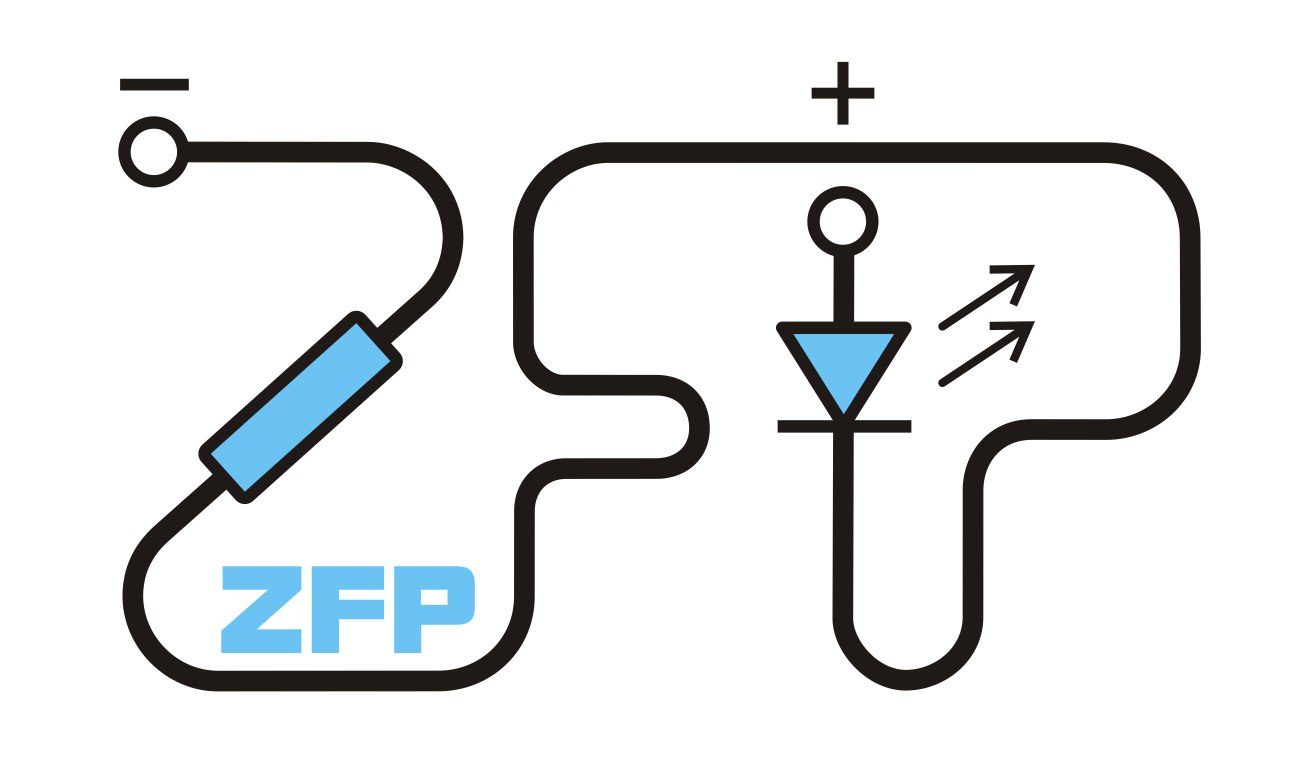
\includegraphics[width=4.5cm]{ZFP.jpg}
\end{center}
\end{minipage}\\\\

%\vspace*{0.5cm}

{
\setstretch{1.5}
\Large
\noindent
Úloha č. \titcislo

\noindent
Název úlohy: \titnazev

\noindent
Jméno: \titjmeno
\hspace*{\fill}
Obor: \titobor

\noindent
Datum měření: \titmereni
\hspace*{\fill}
Datum odevzdání: \titodevzdani

\phantom{d}
}
\end{minipage}
}
%Konec horního rámečku

{
\phantom{d}

\Large
Připomínky opravujícího:\\
\vspace*{6.75cm}
}

\newcommand{\linka}{\noalign{\hrule height 1pt}}
\newcommand{\linkadva}{\noalign{\hrule height 1.5pt}}
\setlength\extrarowheight{9.5pt}
\Large
\noindent
\begin{tabular}{!{\vrule width 1.5pt} l !{\vrule width 1pt} c !{\vrule width 1pt} c !{\vrule width 1.5pt}}
\linkadva
   & Možný počet bodů & Udělený počet bodů \\\linkadva
  Práce při měření & 0-3 &  \\\linka
  Teoretická část & 0-2 &  \\\linka
  Výsledky a zpracování měření & 0-9 &  \\\linka
  Diskuse výsledků & 0-4 &  \\\linka
  Závěr & 0-1 &  \\\linka
  Použitá literatura & 0-1 &  \\\linkadva
  \hspace*{\fill} \textbf{Celkem} \hspace*{\fill}& max. 20 &  \\
\linkadva
\end{tabular}
\phantom{d}

Posuzoval: \hspace*{\fill}dne:~~~~~~~~~~~~~~~~~

}%Konec uzavření titulky
\newpage
\newgeometry{top = 2cm, bottom = 2cm, left = 2cm, right = 2cm}
\setcounter{page}{1}
\setmainfont{Linux Libertine O}




\section{Pracovní úkoly}
\begin{enumerate}

    \item Zpracujte přibližně 50 událostí z detektoru ATLAS programem HYPATIA.
    \item Pomocí programu ROOT zobrazte histogram invariantních hmotností pro různě velké statistické soubory.
    \item Identifikujte výrazné píky a přiřaďte je očekávaným částicím.
    \item Zjistěte chybu střední hodnoty invariantní hmotnosti Z bosonu pro různě velké statistické soubory.
    \item Vyneste zjištěné chyby do grafu jako funkci počtu událostí a srovnejte je s očekávanou závislostí.
    \item Interpretujte výsledky statistického testu pro nové částice a rozhodněte, jestli byl učiněn objev.

\end{enumerate}

\section{Teoretická část}
Úloha A1 spočívá v analýze dat ze simulace detektoru ATLAS Velkého hadronového urychlovače (\textit{LHC}). V LHC dochází k vysokoenergetickým srážkám dvou částic, jejichž interakce může produkovat exotické částice s velkou hmotností a krátkou dobou rozpadu. Přestože životnost takových částic typicky nestačí ani na to, aby doletěly z místa srážky do detektoru, můžeme je identifikovat podle jejich specifických rozpadových produktů a klidových hmotností.

\subsection{Bosony \texorpdfstring{$Z$, $H$}{Z, H}}
Nás budou zajímat především bosony $Z^0$ a $H^0$, jejichž typické rozpady jsou následující:
\begin{align*}
    Z^0 &: e^- + e^+ \\
    Z^0 &: \mu^- + \mu^+ \\
    H^0 &: 2 \, Z^0 \\
    H^0 &: 2 \, \gamma
\end{align*}
Toto nejsou zdaleka jediné možné rozpady, ale jsou pro nás nejsnáze detekovatelné. Klidové hmotnosti těchto bosonů~jsou [1]:
\begin{align*}
    m(Z^0) &= (91.188 \pm 0.002) \U{GeV/c^2} \\
    m(H^0) &= (125.09 \pm 0.24) \U{GeV/c^2} \\
\end{align*}
Další částice s podobnými rozpady, které budeme schopni detekovat, jsou mezony $\Jpsi$ (\textit{charmonium}, vázaný stav $c\overline c$) a $\Upsilon$ (\textit{bottomonium}, vázaný stav $b\overline b$). Jejich klidové hmotnosti jsou [1]:
\begin{align*}
    m(\Jpsi) &= (3.096900 \pm 0.000006) \U{GeV/c^2} \\
    m(\Upsilon) &= (10.5794± \pm 0.0012) \U{GeV/c^2} \\
\end{align*}

\subsection{Klidová hmotnost}
Z předchozího je zřejmé, že pro rozlišení těchto částic z rozpadových produktů bude důležité určit klidovou hmotnost. Protože se ale částice pohybují relativistickými rychlostmi, nestačí pouze sečíst klidové hmotnosti produktů. Místo toho máme k dispozici vztah ze speciální relativity:
\begin{equation}
    E^2 = \big( pc \big)^2 + \big( m_0 \, c^2 \big)^2 \: ,
    \label{energy-momentum-rel}
\end{equation}
kde $E$ je energie částice, $p$ její hybnost a $m_0$ klidová hmotnost. V případě rozpadových produktů umíme jejich energii přímo změřit a jejich klidovou hmostnost určíme z toho, o jaký druh částice se jedná. Z \eqref{energy-momentum-rel} tedy umíme dopočítat hybnost rozpadové částice. Díky zákonům zachování energie a hybnosti potom z těchto rozpadových produktů můžeme rekonstruovat klidovou hmotnost původní částice. Pro mnohočásticový systém totiž platí:
\begin{equation*}
    \Big( \sum_n E_n \Big)^2 = \Big( \sum_n p_n \, c \Big)^2 + \big( M_0 \, c^2 \big)^2 \: ,
\end{equation*}
kde $E_n$ jsou energie jednotlivých částic, $p_n$ jsou jejich hybnosti a $M_0$ je klidová hmotnost celého systému, a tedy i původní částice. Snadnou úpravou dostáváme:
\begin{equation}
    M_0 = \frac{1}{c^2} \, \sqrt{
        \Big( \sum_n E_n \Big)^2 -
        \Big( \sum_n p_n \, c \Big)^2
    }
    \: .
    \label{rest-mass}
\end{equation}
Ačkoliv rovnice \eqref{rest-mass} umožňuje rekonstrukci z obecného mnohačásticového rozpadu, nejspolehlivější je určení původní částice z páru rozpadových částic.

\phantom{.}
\begin{wrapfigure}{r}{8cm}
    \vspace{-2\baselineskip}
    \centering
    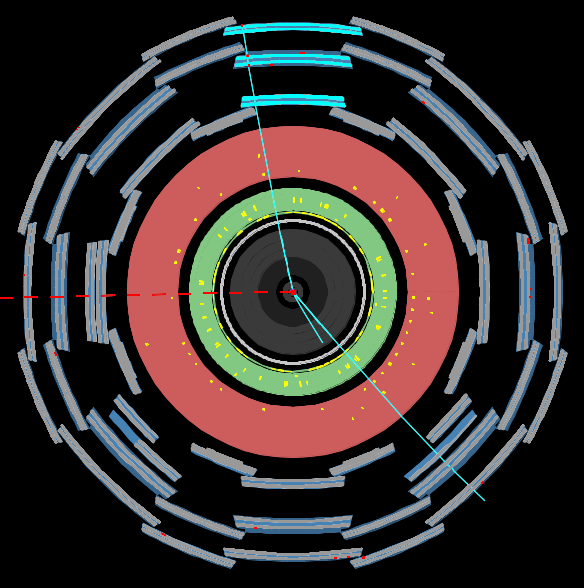
\includegraphics[width=7cm]{detektor.png}
    \caption{Příčný řez detektorem ATLAS}
    \label{obr:detektor}
\end{wrapfigure}

\vspace{-2\baselineskip}
\subsection{Identifikace částic}
Data z detektoru budeme analyzovat v programu HYPATIA, který nám umožňuje zobrazit dráhy detekovaných částic na příčném a podélném řezu detektoru. Příčný řez je možné vidět na obrázku \ref{obr:detektor}.

Detektor se skládá ze čtyř podstatných částí: vnitřní části (na obrázku šedá) s magnetickým polem, které zakřivuje dráhu nabitých částic, elektromagnetického kalorimetru (na obrázku zelená), kde je absorbována energie elektromagnetických spršek, hadronový kalorimetr (na obrázku červená) a nakonec mionová komora (na obrázku šedomodrá\footnote{Jsou-li ve vašem prohlížeči PDF jiné barvy, než jaké jsou zde uvedeny, autor se vám omlouvá. Jedná se o technický problém, který se mu ani přes vynaloženou snahu nepodařilo eliminovat. Pokud jsou barvy tak moc k nepoznání, že vám to znemožňuje identifikaci jednotlivých částí, vězte, že jsou části detektoru vyjmenovávány v pořadí ze středu směrem ven. Pokud je jedna z barev, které vidíte, oktarínová, kontaktujte prosím autora a jako přílohu mu zašlete detailní informace o vašem systému a fyzickou fotografii monitoru.}), do které z detekovatelných částic doletí pouze miony.

My se budeme pokoušet pouze o identifikaci párů elektron-pozitron, jejichž dráha typicky končila už v rámci vnitřní části, foton-foton, které byly detekovány v elektromagnetickém kalorimetru, a mion-antimion, které proletěly celým detektorem až do mionové komory.


\section{Výsledky měření}

\subsection{Události identifikované autorem}
Z dostupných dat se nám podařilo identifikovat celkem 47 rozpadů na $e^- + e^+$, $\mu^- + \mu^+$ nebo $2 \, \gamma$. Kritériem při určování bylo, zda je možné jednoznačně identifikovat, že obě částice vylétají z jednoho bodu, a tedy mohou být produktem jednoho rozpadu. Pokud z jednoho bodu vylétaly tři částice a nebylo zřejmé, které patří do jednoho rozpadového páru, tuto událost jsme přeskočili. Podařilo se také identifikovat celkem tři čtyřčásticové rozpady.

Z identifikovaných srážek jsme vypočítali invariantní hmotnosti potenciálních rozpadlých částic. Jak je vidět z obrázku \ref{obr:c0-full}, počty událostí jsou v řádu jednotek a většina energetického spektra má pouze osamocené události. Jediný zajímavý pík je kolem ${\sim} 100 \U{GeV}$, detailnější histogram tohoto píku najdeme na obrázku \ref{obr:c0-Z}.

\begin{figure}[h]
    \centering
    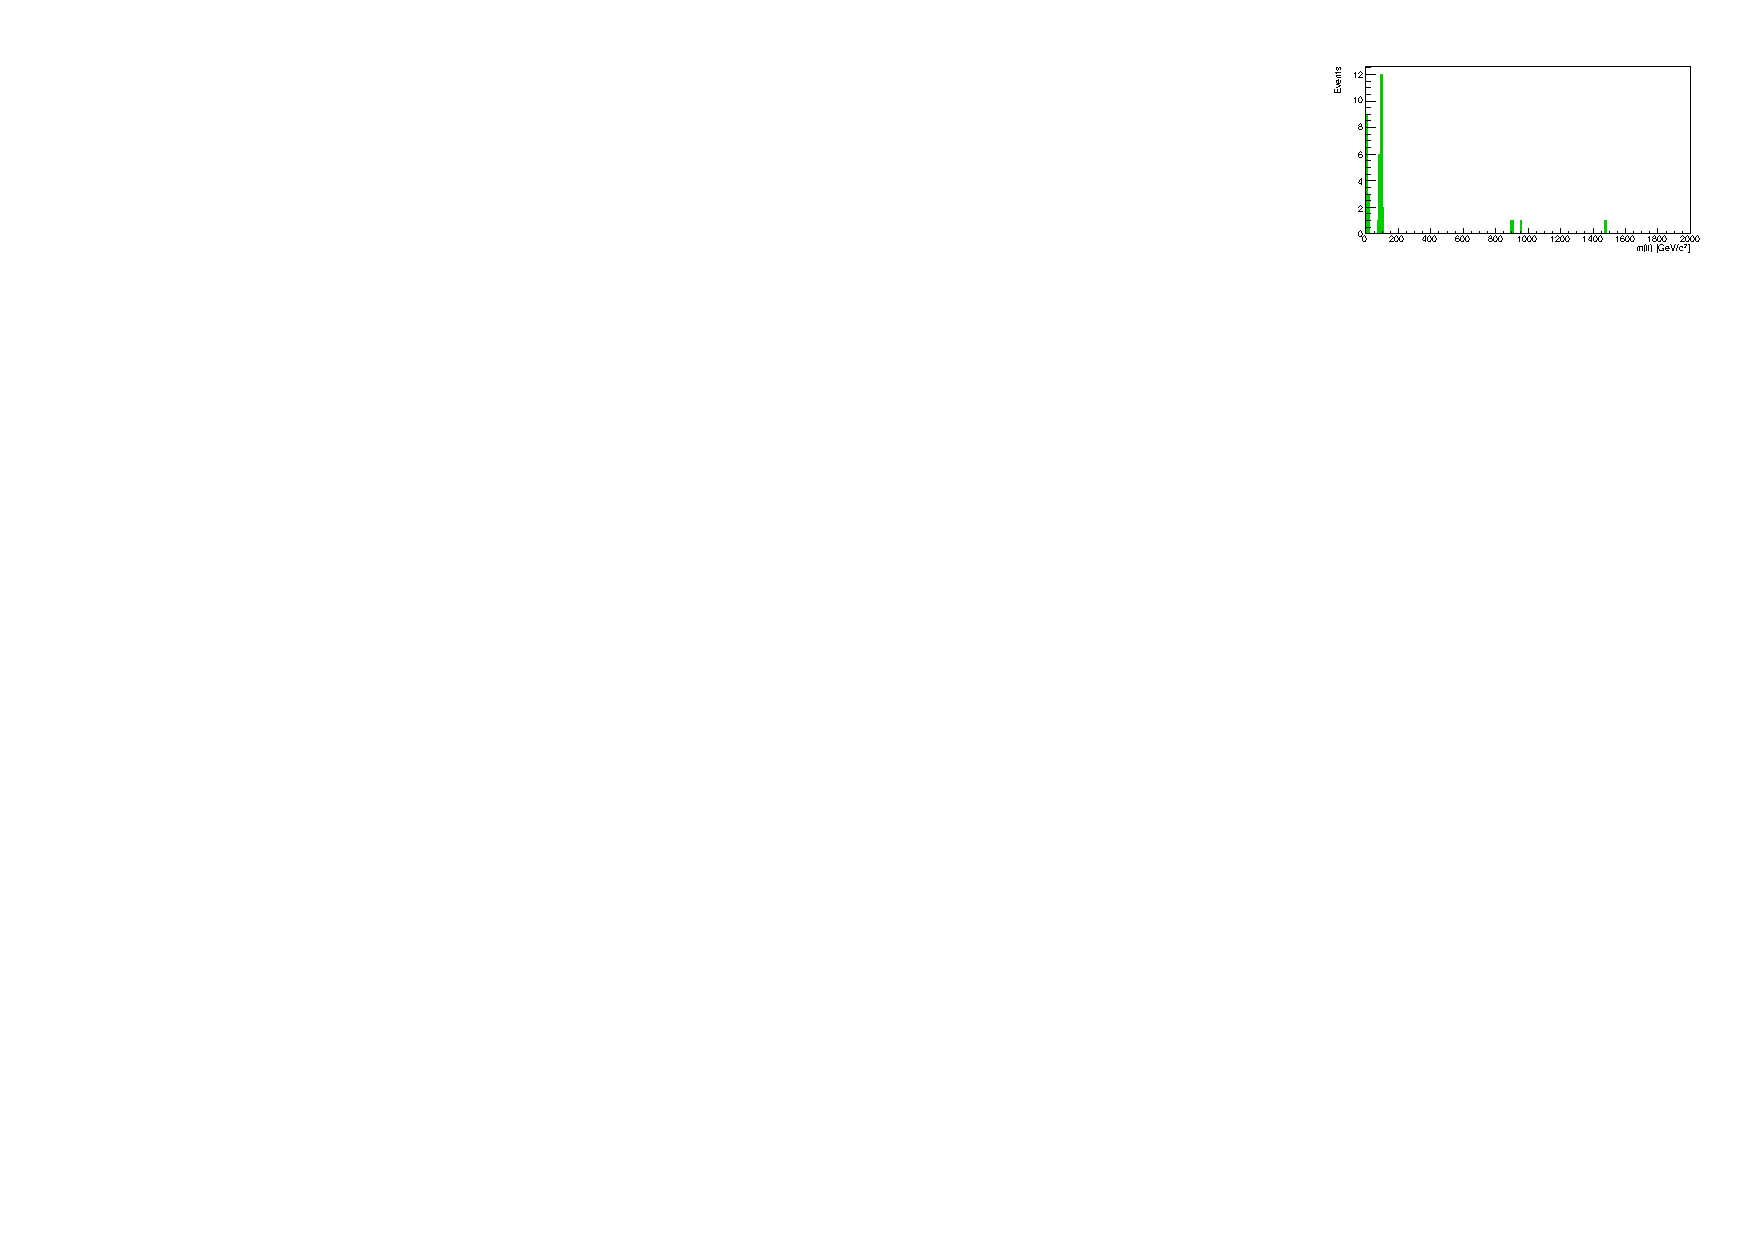
\includegraphics[width=0.6\textwidth]{c0_full.pdf}
    \vspace{-\baselineskip}
    \caption{Histogram všech vypočátaných $M_0$ z autorem identifikovaných srážek.}
    \label{obr:c0-full}
\end{figure}

\noindent
Fitem tohoto píku jsme získali invariantní hmotnost
\begin{align*}
    M_0 = (88.2 \pm 3.3) \U{GeV/c^2} \: ,
\end{align*}
což je v souladu s hmotností $Z$ bosonu. Také jsme detekovali vyšší množství událostí v oblasti jednotek GeV – ty pravděpodobně pochází z rozpadů mezonů $\Jpsi$ a $\Upsilon$, počet událostí je ovšem příliš nízký na to, aby se dal rozumně proložit fitem.

\begin{figure}[h]
    \centering
    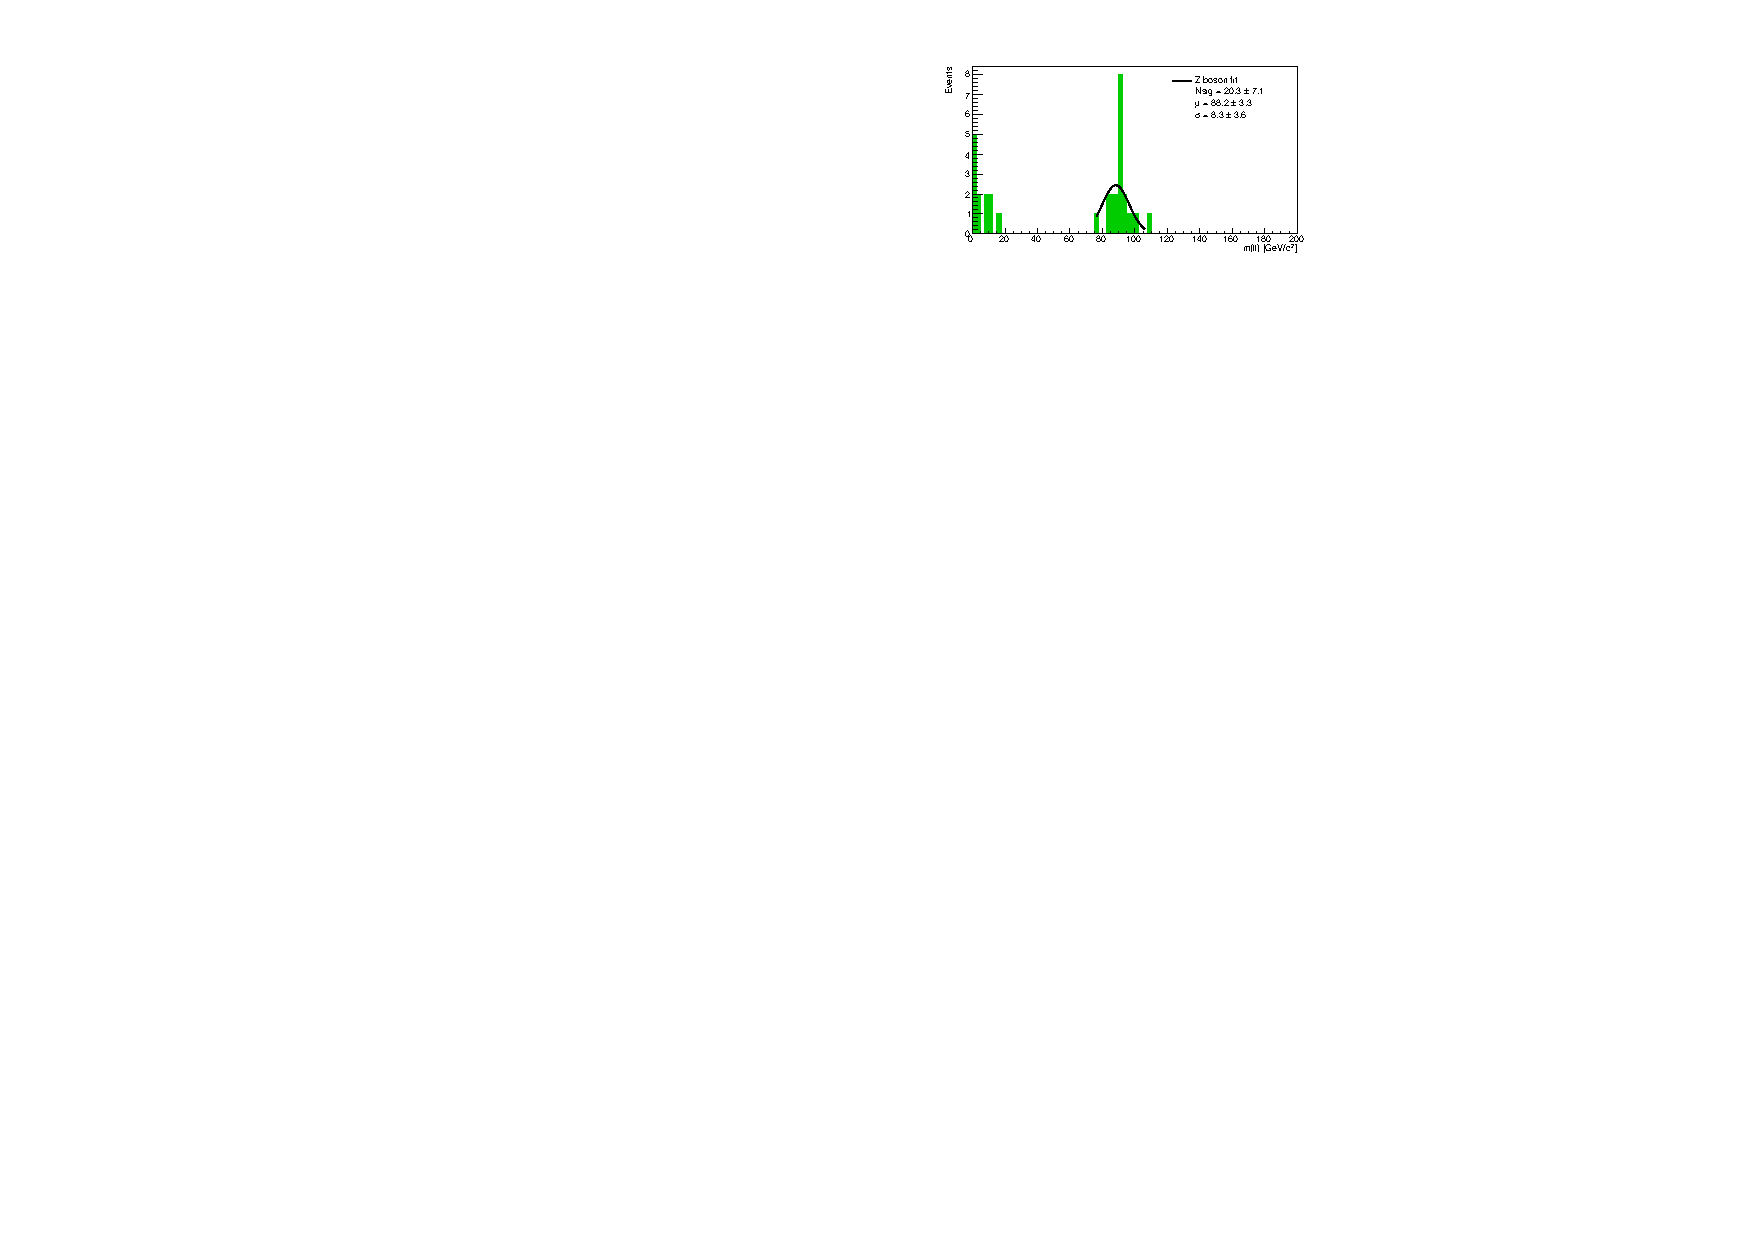
\includegraphics[width=0.6\textwidth]{c0_Z.pdf}
    \vspace{-\baselineskip}
    \caption{Histogram vypočátaných $M_0$ v okolí píku.}
    \label{obr:c0-Z}
\end{figure}


\subsection{Soubor dat od různých autorů}
V rámci praktika se shromažďují události identifikované všemi studenty, kteří se úlohy A1 účastní. Tento soubor obsahuje o několik řádů vyšší počet identifikovaných událostí, proto umožňuje identifikaci píků, které jsme ve vlastních datech nemohli pozorovat.

Na obrázku \ref{obr:c1-full} vidíme všechna data odpovídající rozpadům na leptonové páry (tj. $e^- \!\!+\! e^+$ a $\mu^- \!\!+\! \mu^+$). Kromě píku kolem $100 \U{GeV/c^2}$ vidíme i píky na $1 \U{TeV/c^2}$, což je přibližně kintetická energie letícího komára [2], a $1.5 \U{TeV/c^2}$. Na obrázku \ref{obr:c1-Z} vidíme detail píku $Z$ bosonu a na obrázku \ref{obr:c1-Y} potom detail píku, který jsme dříve neidentifikovali a který odpovídá mezonu $\Upsilon$.

\begin{figure}[h]
    \centering
    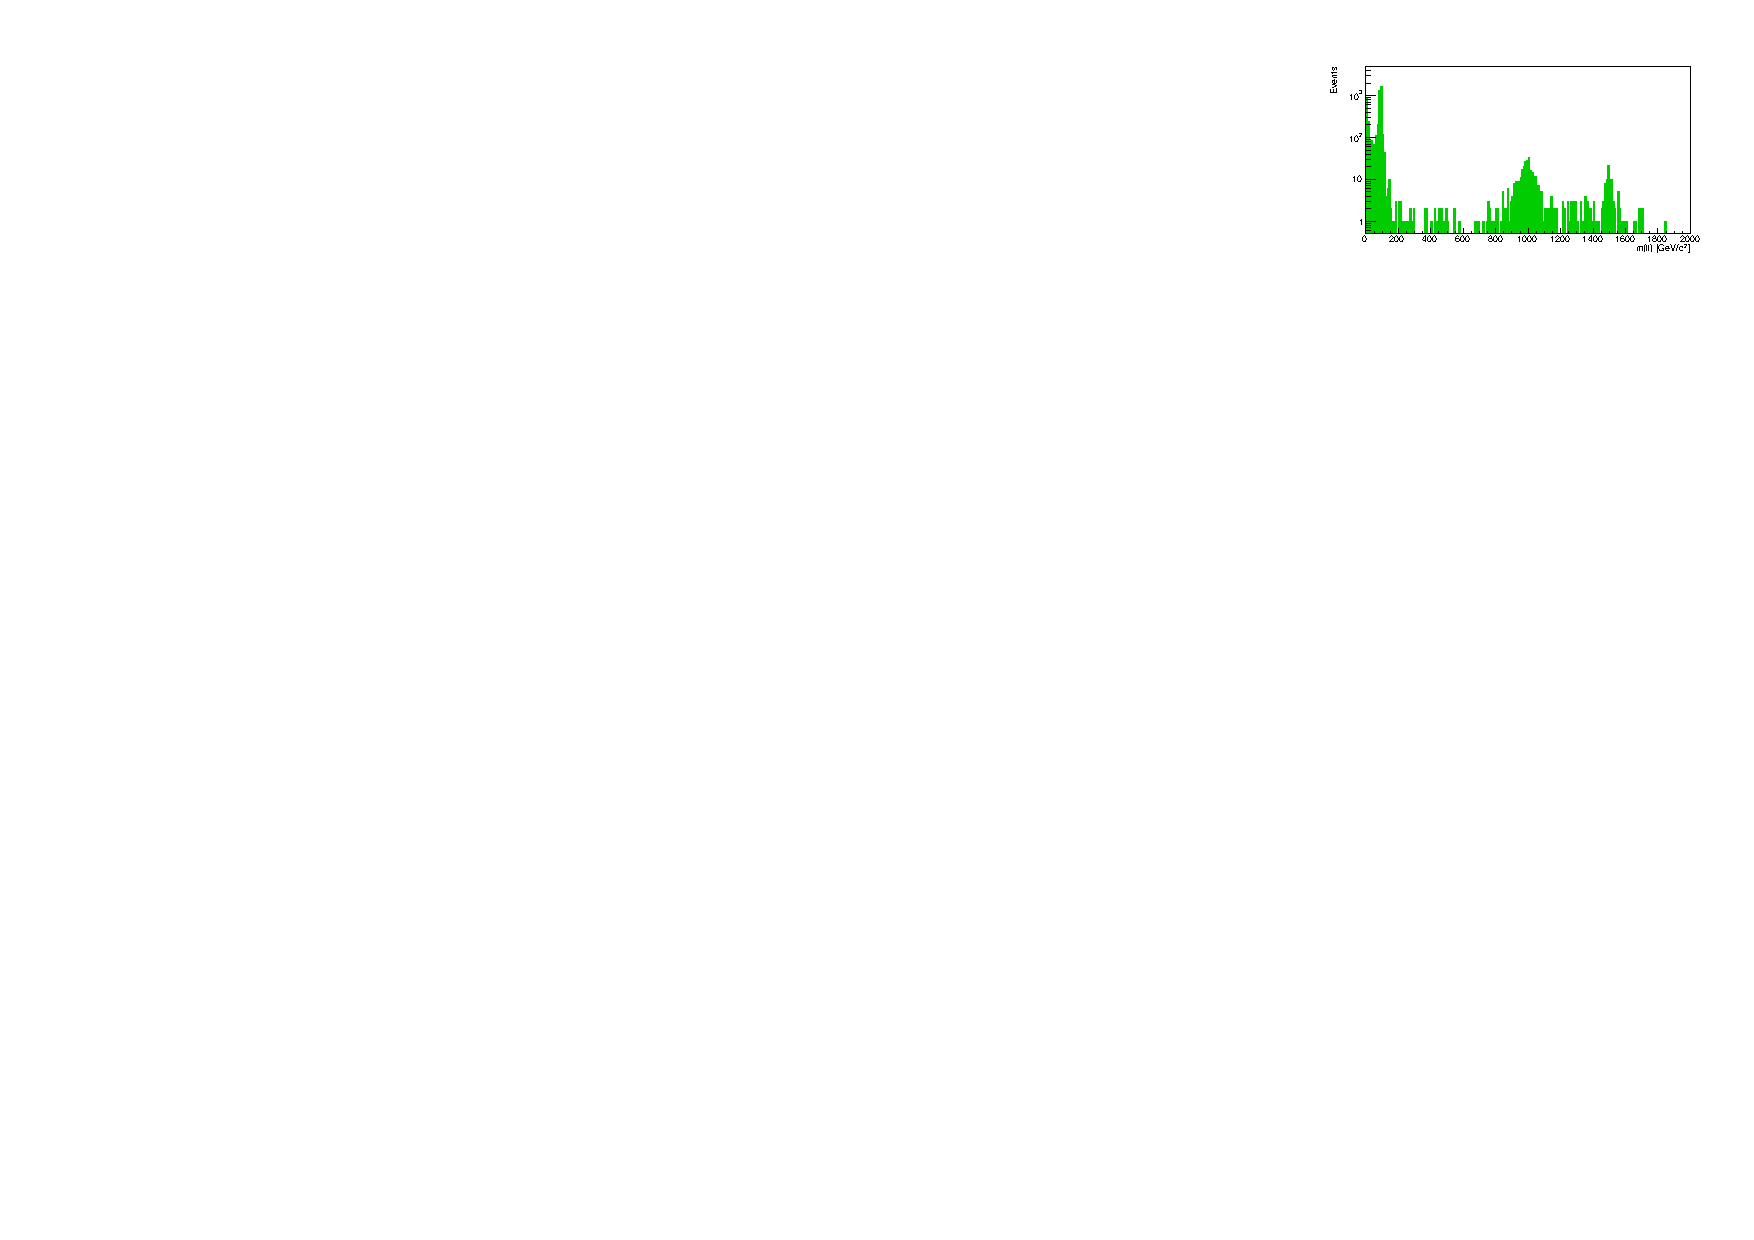
\includegraphics[width=0.6\textwidth]{c1_full.pdf}
    \vspace{-\baselineskip}
    \caption{Histogram všech $M_0$ vypočítaných z leptonových párů.}
    \label{obr:c1-full}
\end{figure}

\begin{figure}[h]
    \centering
    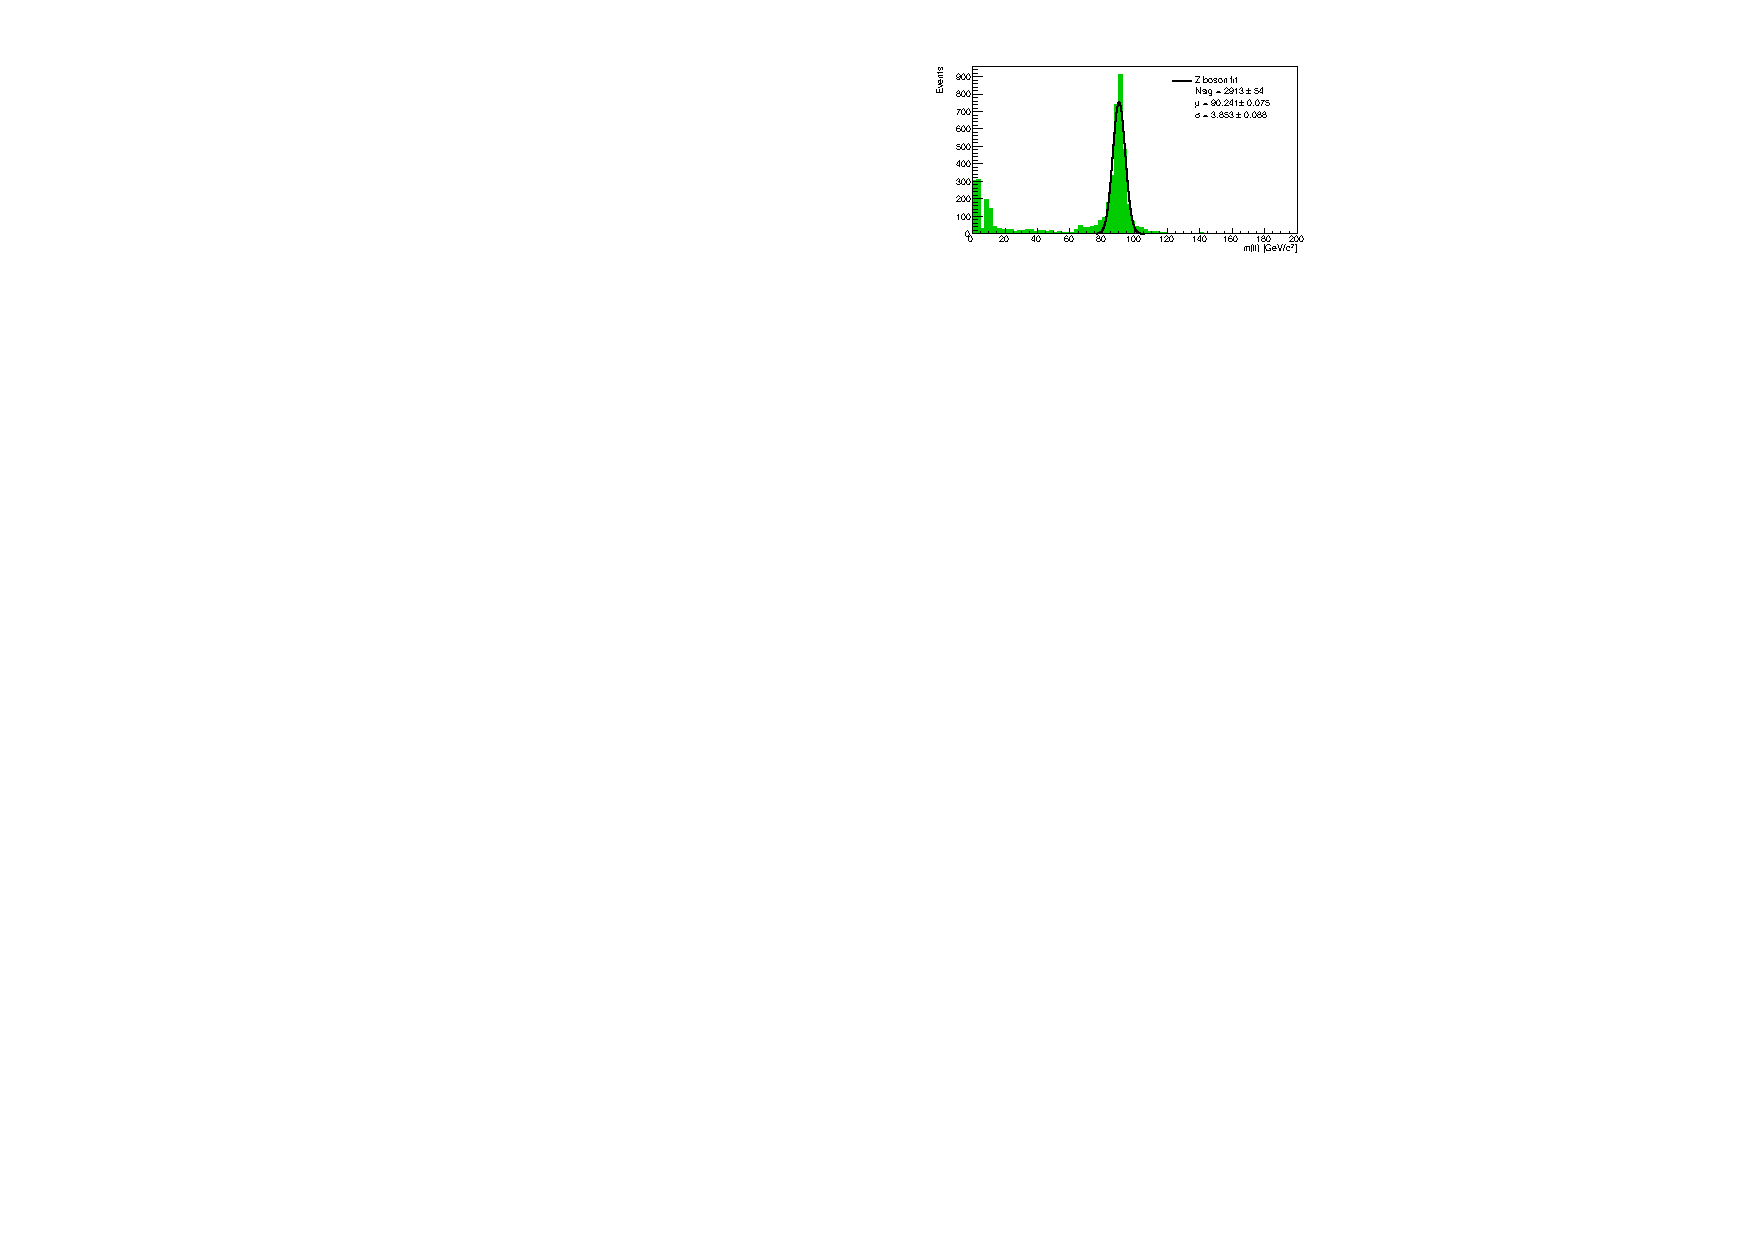
\includegraphics[width=0.6\textwidth]{c1_Z.pdf}
    \vspace{-\baselineskip}
    \caption{Detail píku $Z$ bosonu, leptonové páry.}
    \label{obr:c1-Z}
\end{figure}

\begin{figure}[h]
    \centering
    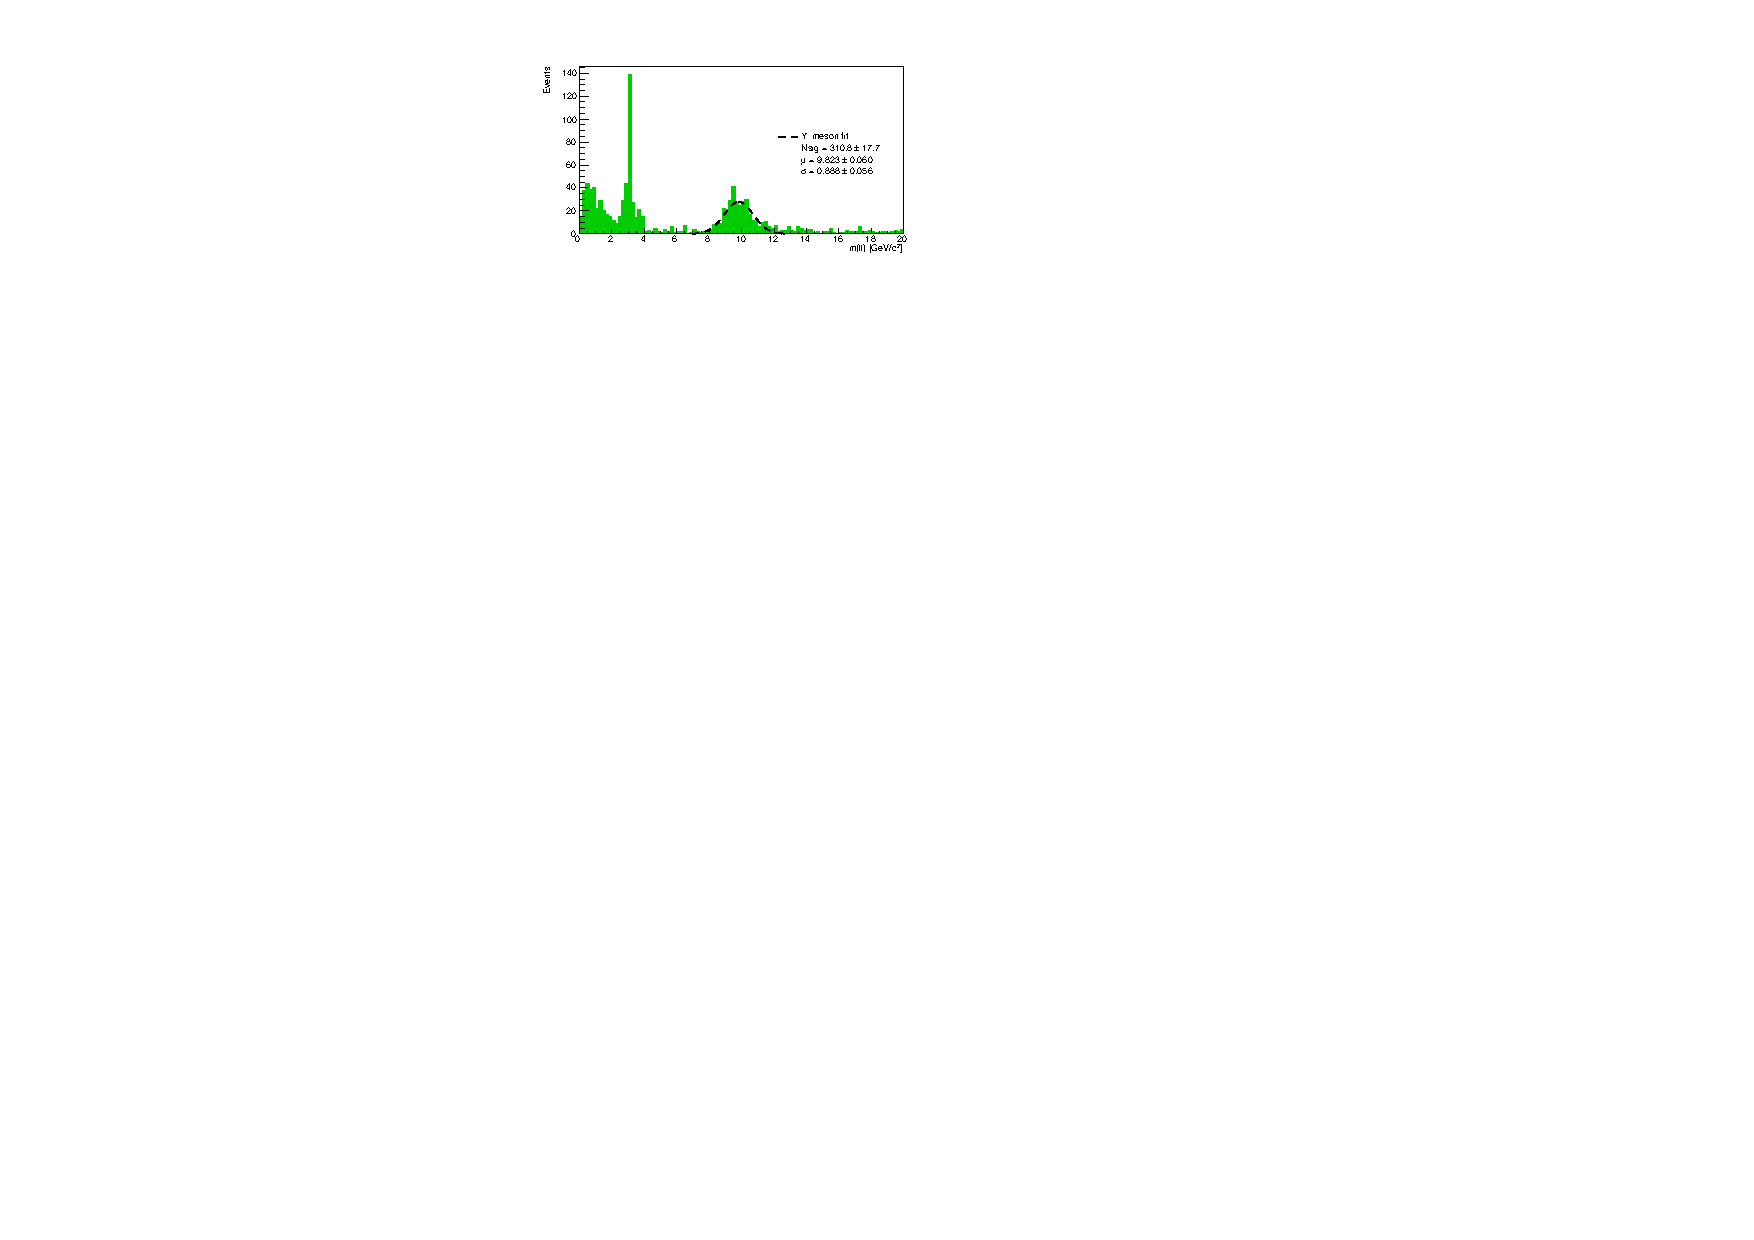
\includegraphics[width=0.6\textwidth]{c1_Y.pdf}
    \vspace{-\baselineskip}
    \caption{Detail píku mezonu $\Upsilon$, leptonové páry.}
    \label{obr:c1-Y}
\end{figure}

\noindent
Pro píky odpovídající $Z$ a $\Upsilon$ jsme provedli fit, střední hodnoty vyšly:
\begin{align*}
    M_0(Z) &= (90.24 \pm 0.08) \U{GeV/c^2} \: , \\
    M_0(\Upsilon) &= (9.82 \pm 0.06) \U{GeV/c^2} \: .
\end{align*}

Porovnáme-li obrázek \ref{obr:c1-full} odpovídající leptonovým rozpadům s obrázky \ref{obr:c1-photons} (fotonové rozpady) a \ref{obr:c1-electrons} (pouze rozpady na elektron-pozitron), můžeme pozorovat několik kvalitativních rozdílů. Píku bosonu $Z$ je v leptonových a elektronových datech velmi podobný, v datech k fotonům je výrazně širší a posunutý k vyšším energiím. Částice s hmotností $1 \U{TeV/c^2}$ vůbec nemá fotonový pík a částici s hmotností $1.5 \U{TeV/c^2}$ zase chybí elektronový pík.

\begin{figure}[h]
    \centering
    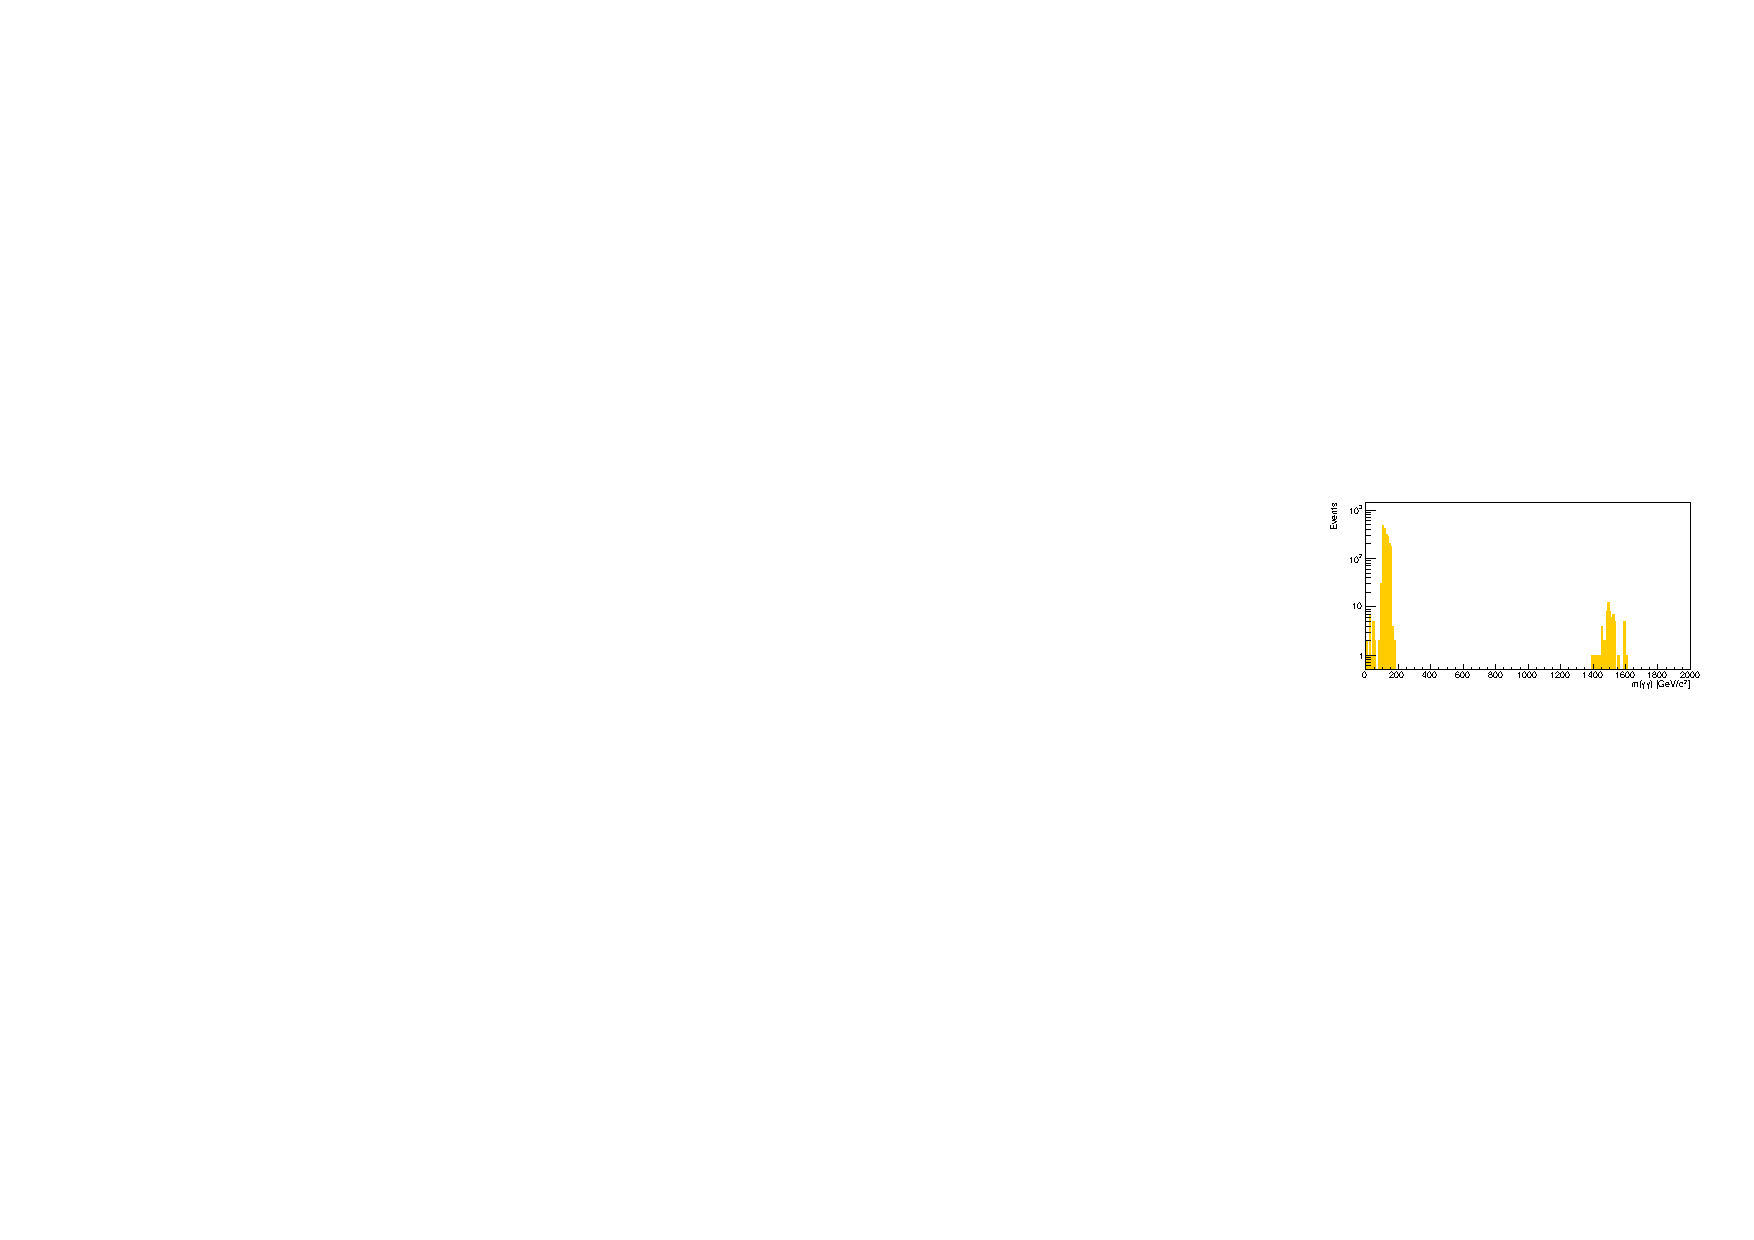
\includegraphics[width=0.6\textwidth]{c1_photons.pdf}
    \vspace{-\baselineskip}
    \caption{Histogram všech $M_0$ vypočítaných z párů fotonů.}
    \label{obr:c1-photons}
\end{figure}

\begin{figure}[h]
    \centering
    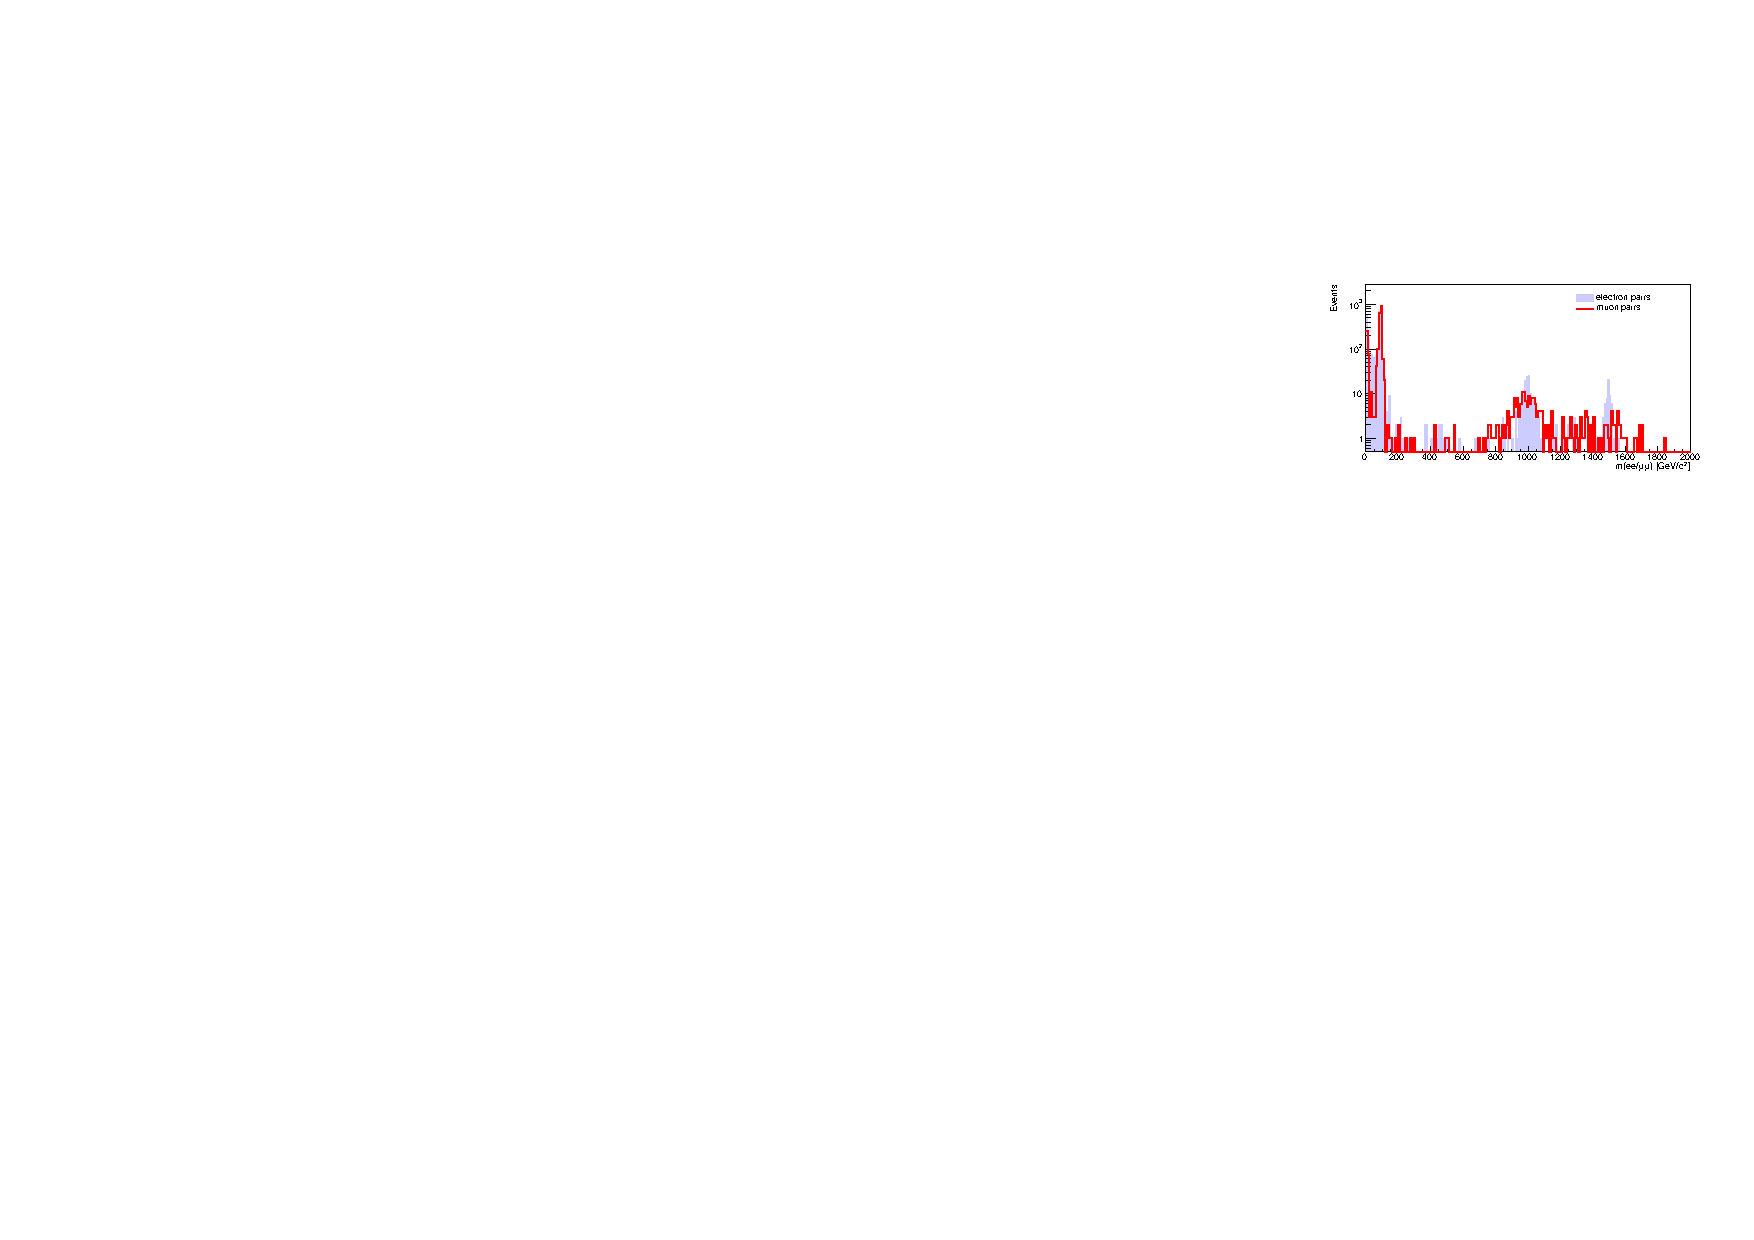
\includegraphics[width=0.6\textwidth]{c1_electrons.pdf}
    \vspace{-\baselineskip}
    \caption{Histogram všech $M_0$ vypočítaných z párů elektron-pozitron.}
    \label{obr:c1-electrons}
\end{figure}

Porovnali jsme statistiku z různě velkých souborů. Předpokládáme, že střední hodnota fitů bude mít chybu nepřímo úměrnou odmocnině z počtu událostí [1]. Skutečnou závislost chyby na počtu událostí jsme vypsali do tabulky \ref{tab:sirka-peak} a vynesli do grafu v obrázku \ref{obr:sirka-peak} společně s fitem předpokládanou závislostí.

\begin{table}[h!]
    \centering
    \begin{tabular}{ r|r }
        \bfseries $N$ & chyba [GeV]
        \csvreader[ head to column names ]{sirka-peak.csv}{}
        {
            \csviffirstrow{\\\hline}{\\} \pocet & \chyba
        }
    \end{tabular}
    \caption{Chyby maxima píku pro $Z$ boson.}
    \label{tab:sirka-peak}
\end{table}

\begin{figure}[h]
    \centering
    \begin{gnuplot}[terminal=epslatex,terminaloptions={color size 9cm, 5cm}]
        set datafile separator ','

        a = 1
        f(N) = a / sqrt(N)

        fit f(x) 'sirka-peak.csv' skip 1 via a
        plot 'sirka-peak.csv' skip 1 t 'data', f(x) t 'fit $a/\sqrt{N}$'
    \end{gnuplot}
    \caption{Chyba střední hodnoty píku $Z$ bosonu vs. počet událostí.}
    \label{obr:sirka-peak}
\end{figure}

\pagebreak

\begin{wrapfigure}{r}{0.4\textwidth}
    \centering
    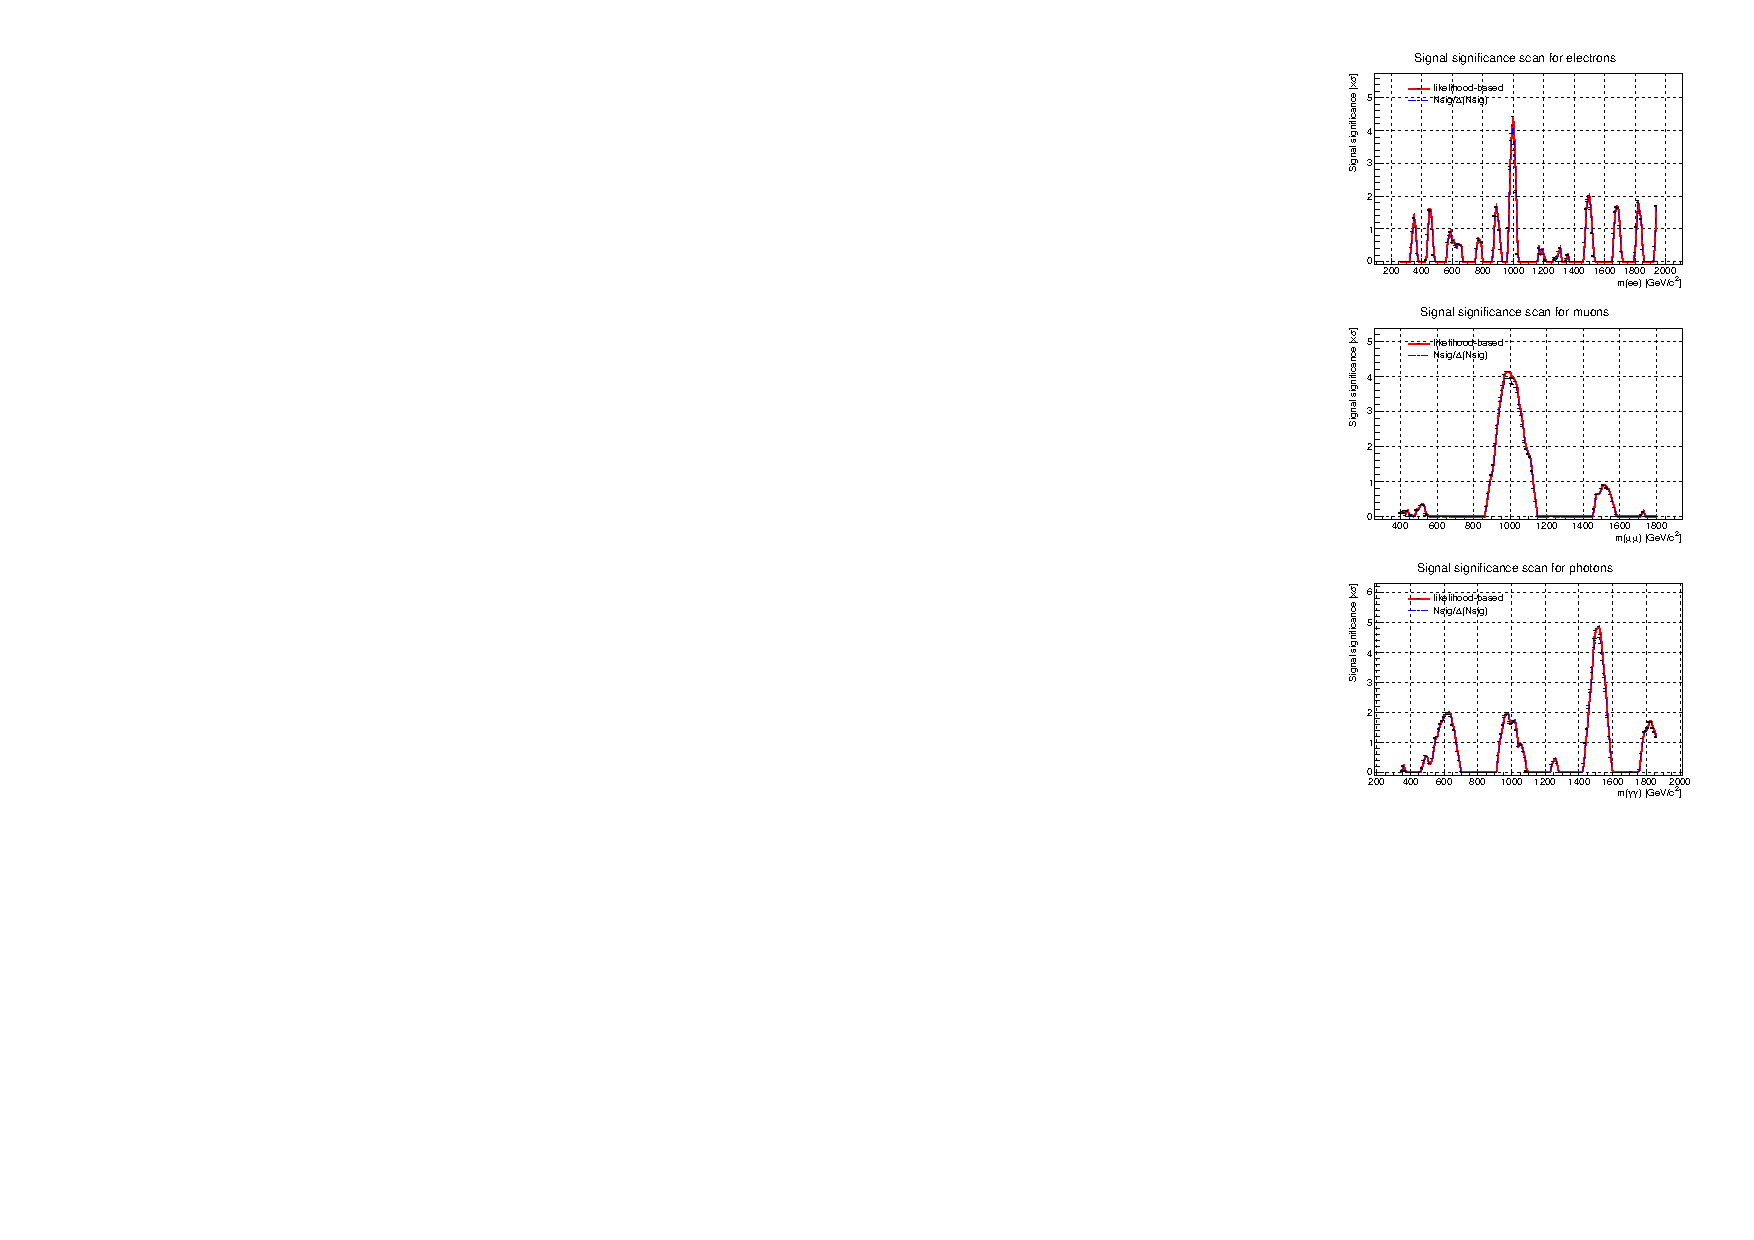
\includegraphics[width=0.4\textwidth]{c4_signif.pdf}
    \vspace{-2\baselineskip}
    \caption{Signifikance jednotlivých píků.}
    \label{obr:signif}
    \vspace{-5cm}
\end{wrapfigure}


Nakonec jsme zkoumali signifikanci naměřených peaků $1 \U{TeV}$ a $1.5 \U{TeV}$. Nulovou hypotézu jsme formulovali tak, že peaky byly způsobeny pouze šumem, ne skutečnou částicí. Standardně se v částicové fyzice požaduje signifikance 5-sigma. Jak je vidět v grafech na obrázku \ref{obr:signif}, této signifikance se nepodařilo dosáhnout ani v jednom případě, ačkoliv pík odpovídající rozpadu foton-foton na $1.5 \U{TeV}$ se této signifikanci blíží. Nulovou hypotézu se tedy nepodařilo vyvrátit a naše data tedy dostatečně neprokázala, že píky nejsou pouze náhodnou fluktuací.


\section{Diskuse}
V datech se podařilo identifikovat dva píky, které neodpovídaly známým částicím. Ačkoliv se nejedná o signifikantní objev podle standardu 5-sigma, je to přesto poměrně přesvědčivá evidence, že by mohly existovat částice s klidovou hmotností $1 \U{TeV/c^2}$ a $1.5 \U{TeV/c^2}$. Lehčí z těchto částic by se rozpadala výhradně na pár lepton-antilepton, těžší z těchto částic na mion-antimion nebo foton-foton. Protože máme o těchto hypotetických částicích pouze velmi málo informací, není snadné určit, jestli odpovídají nějaké teoretické předpovědi. Mohlo by jít o $Z'$ boson a graviton. Nebo by mohlo jít o částice supersymetrické teorie, které mají srandovní jména: třeba smeson tvořený sstrange squarkem a jeho antičásticí, nebo například gaugino bosino wino, což je jedno ze tří hypotetických electroweakin\footnote{Autorův skromný názor je, že částice s takovými názvy by nikdy neměly existovat, a tudíž je neúspěch SUSY pro částicovou fyziku dobrý.}.

V grafu \ref{obr:sirka-peak} skutečná data neodpovídala přesně teoretické závislosti. To mohlo být způsobeno například tím, že jsme nepočítali jenom události v píku, ale i v šumu kolem.

\vspace{3.2cm}

\pagebreak

\section{Závěr}
Podařilo se zpracovat události ze simulace detektoru ATLAS a ze zpracovaných dat se podařilo určit invariantní hmotnost bosonu $Z$ jako:
\begin{equation*}
    m(Z) = (88.2 \pm 3.3) \U{GeV/c^2} \: .
\end{equation*}
Dále se ze souboru dat od různých autorů podařilo zpřesnit hmotnost $Z$ a určit hmotnost $\Upsilon$:
\begin{align*}
    m(Z) &= (90.24 \pm 0.08) \U{GeV/c^2} \: , \\
    m(\Upsilon) &= (9.82 \pm 0.06) \U{GeV/c^2} \: .
\end{align*}
Také se podařilo identifikovat dvě potenciální neznámé částice, ačkoliv se nejedná o objev se signifikancí 5-sigma.



\section{Literatura}
[1] Praktikum částicové a jaderné fyziky. Objevování částic v detektoru ATLAS v CERN. Dostupné z: \url{https://physics.mff.cuni.cz/vyuka/zfp/_media/zadani/texty/txt_401.pdf}. 26. září 2019
\\\\
{}[2] Přispěvatelé Wikipedie. Electronvolt. Wikipedia, The Free Encyclopedia. Citováno 2. 12. 2020. Dostupné z: \url{https://en.wikipedia.org/wiki/Electronvolt}

\end{document}
